\documentclass[12pt, twoside]{article}
\documentclass[12pt, twoside]{article}
\usepackage[letterpaper, margin=1in, headsep=0.2in]{geometry}
\setlength{\headheight}{0.6in}
%\usepackage[english]{babel}
\usepackage[utf8]{inputenc}
\usepackage{microtype}
\usepackage{amsmath}
\usepackage{amssymb}
%\usepackage{amsfonts}
\usepackage{siunitx} %units in math. eg 20\milli\meter
\usepackage{yhmath} % for arcs, overparenth command
\usepackage{tikz} %graphics
\usetikzlibrary{quotes, angles}
\usepackage{graphicx} %consider setting \graphicspath{{images/}}
\usepackage{parskip} %no paragraph indent
\usepackage{enumitem}
\usepackage{multicol}
\usepackage{venndiagram}

\usepackage{fancyhdr}
\pagestyle{fancy}
\fancyhf{}
\renewcommand{\headrulewidth}{0pt} % disable the underline of the header
\raggedbottom
\hfuzz=2mm %suppresses overfull box warnings

\usepackage{hyperref}
\usepackage{float}

\title{Algebra 2}
\author{Chris Huson}
\date{June 2024}

\fancyhead[LE]{\thepage}
\fancyhead[RO]{\thepage \\ Name: \hspace{1.5cm} \,\\}
\fancyhead[LO]{BECA/Huson/Algebra 2: Regents Preparation \\* 13 June 2024}

\begin{document}
\subsubsection*{Prep - graphing stationary}
\begin{enumerate}
\item Best practices for Regents graphing problems:
    \begin{itemize}[label=$\square$, itemsep=0.25cm]
        \item Use the calculator graph and table functions.
        \item Set the window (F3) based on the equation and grid numbering.
        \item Mark and label the $x$-intercepts.
        \item Note maxima and minima, drawing smooth curves.
        \item Add arrows unless the domain is restricted.
    \end{itemize}
    \begin{center}
        \begin{tikzpicture}[scale=0.7]
        \draw[gray,thin] (-10,-10) grid[xstep=1,ystep=1] (10,10);
        \draw [thick,->] (-10,0)--(10.3,0) node [above] {$x$};
        \draw [thick,->] (0,-10)--(0,10.5) node [above] {$y$};
        \end{tikzpicture}
        \end{center}

\newpage
    \begin{center}
    \begin{tikzpicture}[scale=0.65]
        \draw[thin,gray] (0,0) grid (15,15);
        \draw[thick,->] (0,0) -- (15.5,0) node[below] {$x$};
        \draw[thick,->] (0,0) -- (0,15.5) node[above] {$f(x)$};
    \end{tikzpicture}
    \end{center}

    \begin{center}
    \begin{tikzpicture}[scale=0.5]
    \draw [thick,->] (-10,0)--(10.3,0) node [above] {$x$};
    \draw [thick,->] (0,-10)--(0,10.5) node [above] {$y$};
    \end{tikzpicture}
    \end{center}

\end{enumerate}
\end{document}